\lab{Исследование вольт-амперной характеристики вакуумного диода}
\aim{определение удельного заряда электрона на основе закона <<трёх вторых>>
    для вакуумного диода.}
\equip{вакуумная лампа с цилиндрическим анодом; амперметр; многопредельные
микроамперметр и вольтметр постоянного тока; стабилизированные источники
постоянного тока и постоянного напряжения.}

Перед выполнением работы необходимо ознакомиться с теоретическим Введением
к разделу (п.~\ref{sec:vac_di}).

%\todo[inline,author=Popov,color=cyan]{Интегрировать в описание работы и там дополнить
%--->}
%Теперь задача о распределении потенциала становится однозначной и приводит к
%решению
%\begin{equation*}
%    j=\frac{4\varepsilon_0}{9x^2}\sqrt{\frac{2e}{m}}\varphi^{3/2}.
%\end{equation*}
%\todo[inline,author=Popov]{Убрать детали в описание работы,
%во введении --- только общие законы}
%
%Так как $\varphi(d)=V$, где~$d$~--- расстояние между электродами, то для
%зависимости тока от напряжения получаем
%\begin{equation*}
%    I=\frac{4\varepsilon_0 S}{9d^2}\sqrt{\frac{2e}{m}}V^{3/2},
%\end{equation*}
%где~$S$~--- площадь катода. Мы получили зависимость тока через плоский диод от
%приложенного к нему напряжения, известную как <<закон трёх вторых>> для плоского
%диода. Оказывается, что не только для плоского вакуумного диода, а и для
%вакуумного диода с электродами любой другой геометрии ток подчиняется <<закону
%степени трёх вторых>>.
%
%Полученная формула подсказывает процедуру измерения удельного заряда электрона.
%Для этого достаточно по
%результатам эксперимента построить график зависимости тока от напряжения в
%степени трёх вторых, который должен
%представлять собой прямую линию, проходящую через начало координат. Угол наклона
%этой прямой линии пропорционален (с известным коэффициентом) квадратному корню
%из~$e/m$~--- искомой величины удельного заряда электрона.
%\todo[inline,color=cyan]{<---}

В~работе исследуется зависимость величины тока, проходящего через вакуумный диод,
от напряжения на нём (положительная ветвь вольт-амперной характеристики).
Наибольший интерес представляет та область значений положительного напряжения
на диоде, для которой пространственный заряд (электронное облако) в лампе 
существенно влияет на распределение электрического поля между катодом и анодом
(\emph{режим пространственного заряда}). Электрическое поле этого заряда
<<экранирует>> поле вблизи катода, из-за чего 
лишь незначительная часть электронов, способных преодолеть энергетический барьер
(<<работу выхода>>) и высвобождаемых из катода, создаёт ток через диод.

%Ток через диод при этом существенно меньше тока эмиссии катода из-за того, 
%что электрическое поле пространственного заряда <<экранирует>> поле,
%создаваемое электродами, препятствуя таким образом движению электронов, 
%испущенных катодом. 

Как показано во Введении к разделу, величина 
тока в этом режиме пропорциональна напряжению на диоде в степени 3/2:
\begin{equation}
\eqmark{IU}
	I\propto U^{3/2}
\end{equation}
(<<\emph{закон трёх вторых}>> Чайлда--Ленгмюра). 
Коэффициент пропорциональности в этой формуле зависит
от удельного заряда электрона $e/m$, что позволяет измерть его величину
по вольт-амперной характеристике диода.

В отличие от задачи о плоском диоде, рассмотренной в п.~\ref{sec:vac_di},
в данной работе используется диод цилиндрической формы.
Вывод соотношений и основные результаты п.~\ref{sec:vac_di} при этом 
сохраняются, 
однако в коэффициенте пропорциональности закона 3/2 появляется
дополнительный множитель, зависящий от размера электродов.


\labsubsection{Обобщение на случай цилиндрической геометрии}
Рассмотрим подробнее задачу о цилиндрическом вакуумном диоде.
Пусть катод имеет форму нити радиусом~$r_{К}$, а анод~--- форму полого 
цилиндра радиусом~$r_{А}$ (рис.~\figref{Scheme of electrodes}). 
Между катодом и анодом имеется разность потенциалов~$U$.
Будем считать, что длина диода~$l$ намного превосходит его радиальные
размеры ($l\gg r_{А}$), так что электрическое поле можно 
считать строго радиальным.

\begin{wrapfigure}{o}{0.30\textwidth}
    \centering
	\pic{0.9\linewidth}{Chapter_3/3_2_1}
	\caption{Расположение электродов в диоде}
	\figmark{Scheme of electrodes}
\end{wrapfigure}

В этом случае вместо уравнения \chaptereqref{3.14} для электрического потенциала 
$\varphi(r)$ необходимо записать уравнение Пуассона в цилиндрических координатах:
\begin{equation}
\frac{d}{dr}\left(r\frac{d\varphi}{dr}\right)=-
\frac{r\rho}{\varepsilon_0},
\eqmark{3.2.1}
\end{equation}
где $\rho(r)$~--- объёмная плотность заряда, зависящая от расстояния до оси. 
Граничные условия возьмём в виде 
\begin{equation}
\eqmark{border_phi}
\varphi(r_{К})=0, \quad\varphi(r_{А}) = U.
\end{equation}

В стационарном случае полный ток, пересекающий цилиндрическую поверхность
радиуса $r_{К}\le r \le r_{А}$, постоянен:
\begin{equation}
I=-2 \pi r \rho v l = \mathrm{const}.
\eqmark{3.2.2}
\end{equation}
Здесь $v$ --- скорость электронов, 
набираемая на пройденной ими разности потенциалов:
\begin{equation}
\eqmark{mv2}
\frac{mv^2}{2} = e (\varphi(r)-\varphi(r_{К})).
\end{equation}
(Напомним, что начальной скоростью вылета электронов из катода мы пренебрегаем,
$mv_0^2/2\ll eU$. Однако малых напряжениях~$U$ вклад начальной скорости
может оказаться существенным и закон 3/2 не будет выполняться.)

Исключая с помощью \eqref{3.2.2} и \eqref{mv2} скорость~$v$ и плотность~$\rho$ 
из уравнения \eqref{3.2.1}, получим
(ср. с \chaptereqref{3.15})
\begin{equation}
\frac{d}{dr}\left(r\frac{d\varphi}{dr}\right)=
\frac{I}{2\pi\varepsilon_0l}\sqrt{\frac{m}{2e\varphi}}.
	\eqmark{3.2.5}
\end{equation}

Таким образом, функция $\varphi(r)$ может быть получена как решение
дифференциального уравнения второго порядка. 
Дополнительным граничным условием для него 
является равнество нулю электрического поля на катоде,
следующее из \emph{неограниченности эмиссионной способности} катода (см. обсуждение
во Введении к разделу):
\begin{equation}
E(r_{К})=\left.\frac{d\varphi}{dr}\right|_{r=r_{К}}=0.
\eqmark{3.2.6}
\end{equation}
%Как правило, в реальных электронных лампах при нормальных рабочих 
%режимах $E$ о`бращается в нуль не на самом катоде, а
%на расстоянии 0,01--0,1~мм от него.
%В~условиях нашего опыта этим расстоянием можно пренебречь.

Отметим, что значение тока~$I$ в правой части уравнения \eqref{3.2.5} 
не является независимой величиной и определяется из 
заданных граничных условий на $\varphi(r)$.

Уравнение \eqref{3.2.5} является нелинейным дифференциальным уравнением,
общее решение которого не выражается в квадратурах. 
Однако даже не выписывая решения \eqref{3.2.5}, можно показать, что <<закон 3/2>> для 
цилиндрического диода выполняется. Воспользуемся для этого соображениями 
\emph{физического подобия}. Пусть нам известно решение~$\varphi_0(r)$ при некотором анодном 
напряжении~$U_{0}$, для которого ток оказался равным~$I_{0}$. 
Сделаем в уравнении \eqref{3.2.5} замену 
\[
\varphi(r) = k\varphi_0(r),\qquad I = k^{3/2} I_0,
\]
где $k$ --- произвольная положительная константа. Получим
\[
k\frac{d}{dr}\left(r\frac{d\varphi_0}{dr}\right)=
\frac{k^{3/2} I_0}{2\pi\varepsilon_0l}\sqrt{\frac{m}{2ek\varphi_0}}.
\]
Видно, что коэффициент $k$ в левой и правой частях сокращается, так что вид уравнения остаётся
неизменным. Граничное условие \eqref{3.2.6} при такой замене останется прежним, 
а вместо \eqref{border_phi} получим $\varphi(r_{А})=kU_0$.
Следовательно, функция $\varphi(r)=k\varphi_0(r)$ является решением задачи для 
тока $I=k I_0$. 
Поскольку $\varphi(r_{А})=U$, исключая множитель $k$, приходим к соотношению
\begin{equation}
I = I_0 \left(\frac{U}{U_0}\right)^{3/2},
\end{equation}
что и представляет собой содержание <<закона 3/2>>. Видно, что 
его применимость не зависит от формы или размера электродов, и ограничивается
только сделанным предположениями: 1)~малость начальных скоростей электронов
и 2)~равенство нулю электрического поля на поверхности катода.

В пределе $r_{А}/r_{К} \to \infty$ ($r_{К} \to 0$) уравнение \eqref{3.2.5} 
имеет аналитическое решение. Подставив в него функцию вида
$\varphi = U\cdot (r/r_{А})^{\alpha}$, найдём, что решение существует 
при $\alpha = 2/3$ и 
\begin{equation}
\eqmark{UI_inf}
I = A_0 U^{2/3},\quad \text{где~} A_0 = 
\frac49  \varepsilon_0 \frac{2\pi l}{r_{А}} \sqrt{\frac{2e}{m}}.
\end{equation}
(ср. с формулой для плоского диода \chaptereqref{IU_flat}).
В~общем случае исследуемый закон может быть представлен следующим образом:
\begin{equation}
I = \alpha A_0 U^{3/2},
\eqmark{3.2.8}
\end{equation}
где~$\alpha$~--- функция отношения $r_{А}/r_{К}$ 
($\alpha\to1$ при $r_{А}/r_{К}\to \infty$), которая может быть найдена 
численным интегрированием уравнения \eqref{3.2.5}. 
Результат вычислений представлен на рис.~\figref{beta}.

\begin{figure}[h]
    \centering
    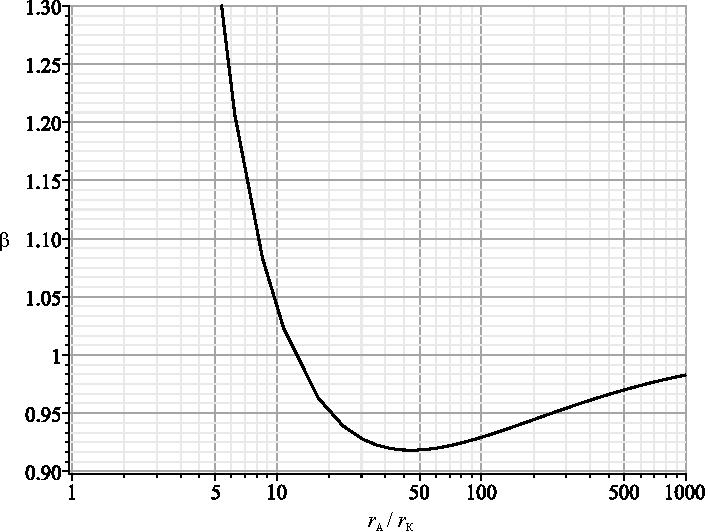
\includegraphics[width=9cm]{beta.pdf}\par
    \caption{Зависимость коэффициента $\alpha$ от отношения радиусов
        электродов~$r_{А}/r_{К}$}
    \figmark{beta}
\end{figure}


\experiment 

Исследования проводятся на диоде с косвенным накалом (ток пропускается через 
расположенную вблизи катода \emph{нить накала}). Радиусы катода~$r_{К}$, 
анода~$r_{А}$, а также длина активной области диода~$l$ 
(участка катода, покрытого оксидным слоем, обеспечивающим
термоэмиссию электронов) указаны на установке. 
Отметим, что длина~$l$ меньше полной длины анода примерно в два раза. 
Благодаря этому рабочая часть катода достаточно 
удалена от его торцов, и следовательно,
электрическое поле в активной части диода с хорошей точностью можно считать радиальным.

Схема экспериментальной установки изображена на рис.~\figref{Scheme}. Для
питания цепи накала и анода используются два регулируемых источника напряжения. 
Ток накала $I_{н}$ измеряется амперметром, включённым последовательно с
балластным сопротивлением $R$. Анодное напряжение~$U$ измеряется вольтметром, 
анодный ток $I$~--- миллиамперметром.
В~работе предлагается измерять анодные токи и напряжения в широком диапазоне 
значений, перекрывающем примерно три порядка величины, 
поэтому вольтметр и миллиамперметр должны быть оснащены устройствами 
ручного или автоматического переключения диапазонов измерения.

\begin{figure}[h!]
    \centering
    \pic{9cm}{Chapter_3/3_2_2}
    \caption{Схема экспериментальной установки}
    \figmark{Scheme}
\end{figure}

\begin{lab:task}

\taskpreamble{В~работе предлагается исследовать вольт-амперные характеристики диода при
различных токах накала и по результатам
измерений определить удельный заряд электрона.}


    
\item Настройте измерительные приборы согласно прилагаемой к установке
инструкции.

\item Перед включением питания установите ручки регулировки источников
в минимальное положение.

\item Установите минимальный ток накала диода~$I_\text{н}$, 
и минимальное значение анодного напряжения~$V_{A}$, 
указанные в инструкции. Дайте лампе прогреться в течение 5--10 минут.

\item\label{l332-p4} Проведите подробные измерения вольт-амперных характеристик диода 
$I(U)$ во всём допустимом диапазоне изменения напряжений  (см. инструкцию
к установке). 

Всего должно быть измерено не менее 25--30 точек, 
не менее чем по 8--10 на каждый диапазон изменения напряжений. 
Как правило, рекомендуется провести и измерения в диапазоне от 0,5 до 50~В, 
при этом для малых напряжений (до 5~В) измерения рекомендуется производить 
с шагом 0,5~В, для средних (до 15~В)~--- с шагом 1~В, и 
для более высоких~--- с шагом 5~В.

\item Повторите измерения вольт-амперных характеристик согласно п.~\ref{l332-p4}
при других величинах тока накала (2--3 значений $I_{н}$).

\tasksection{Обработка результатов}

\item По результатам проведенных измерений постройте 
вольт-амперные характеристики диода 
в двойном логарифмическом масштабе
$\log I (\log U)$
для каждого тока накала. По графикам определите участки, на которых
выполняется <<закон 3/2>>.

\item Используя данные, соответствующие участкам применимости
<<закона 3/2>>, постройте для каждого тока накала вольт-амперные 
характеристики в координатах $I(U^{3/2})$. 
Убедитесь в том, что зависимость является линейной. 

\item Найдите наклоны прямолинейных участков зависимости
$I(U^{3/2})$. Используя формулы \eqref{UI_inf}, \eqref{3.2.8}, 
определите удельный заряд электрона~$e/m$.

\item Оцените погрешность измерений и 
сравните результат измерений с табличным значением.

\end{lab:task}


\begin{lab:questions}
    
    \item Каковы условия применимости <<закона 3/2>> для вакуумного диода?
    Почему закон неприменим при малых и больших напряжениях?
    
    \item Изобразите качественно зависимость тока диода от напряжения
    во всём диапазоне положительных напряжений $U_{А}>0$ на аноде.
    
	\item Нарисуйте качественные графики распределения потенциала $\varphi(r)$ 
    между катодом и анодом: а)~в режиме объёмного заряда;
б)~в режиме насыщения тока диода. Объясните эти зависимости.

    \item Как выглядит вольт-амперная характеристика диода при отрицательных
    напряжениях на аноде, $U_{А}<0$?

	\item Как влияет ток накала катода на ток диода при неизменном напряжении
на аноде? Приводит ли это к погрешности измерения~$e/m$?

    \item Получите уравнение \eqref{3.2.1} из интегральной формы теоремы Гаусса
    для электрического поля.
    
    \item Оцените, при каком токе через диод нельзя пренебрегать
    действием магнитного поля этого тока на движение электронов.

\end{lab:questions}

\begin{lab:literature}
    \item \Kirichenko~--- \S~2.4.
	\item \SivuhinIII~--- \S\S~100--102.
	\item \Kalashnikov~--- \S~157.
\end{lab:literature}

